\section{Aufbau}
\label{sec:Aufbau}
Der Aufbau wird in Abbildung \ref{setup} gezeigt.
\begin{figure}[hp]
    \centering
    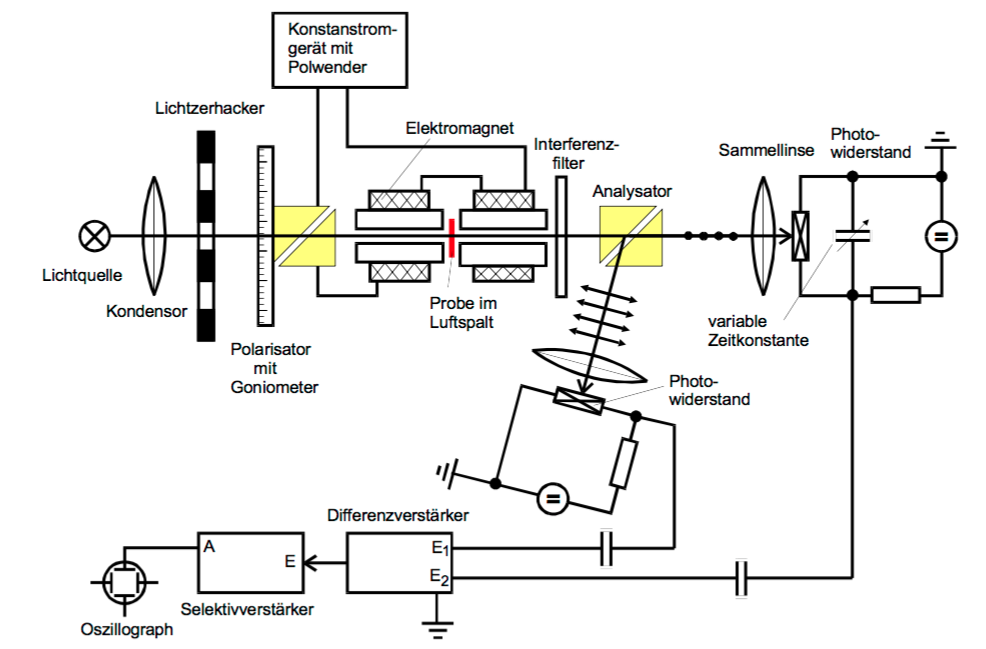
\includegraphics[width=0.9\textwidth]{graphics/setup.png}
    \caption{Trolololo \cite{skript}}
    \label{setup}
\end{figure}
Licht einer Halogenlampe fällt auf einen Interferenzfilter und Analysator,
wodurch der Strahl in zwei senkrecht zueinander linear-polarisierte Strahlen bei einer bestimmten Wellenlänge aufgespalten wird.
Die Wellenlängen-Beschränkung ist notwendig, weil die folgenden optischen Geräte für ein breites Lichtspektrum durchlässig sind,
während die Probe hauptsächlich für Infrarotes Lich durchsichtig ist.
Daher stammt Licht außerhalb vom infraroten Bereich nicht von der Probe und sollte zwecks der Messgenauigkeit gefiltert werden.
Die beiden Teilstrahlen aus dem Analysator werden auf zwei Photowiderstände fokussiert,
deren Leitfähigkeit als Maß für die Polarisationsänderung genommen werden kann.
Liegt eine Polarisation des einfallenden Lichtes vor, die in zwei gleich intensive Teile gespalten wird,
kann an den Dioden die gleiche Spannung gemessen werden.
Um den Aufwand gering zu halten, werden nicht beide Signale der Dioden, sondern die Differenz der Signale gemessen.
Es gilt entsprechend, dass ein Nullsignal eine Polarisation mit zwei gleichen (senkrechten) Polarisationsanteilen anzeigt.
Das Licht der Halogenlampe ist im Allgemeinen nicht polarisiert.
Um die Faraday-Drehung messen zu können, wird vor dem Probenhalter ein Polarimeter mit präzisem Winkelmesser (Goniometer) installiert.

Da das Experiment bei Tageslicht durchgeführt werden soll
und somit Streulicht und Rauscheffekte der Photodioden reduziert werden muss,
wird das einfallende Licht mittels Chopper zu einem Rechtecksignal einer bestimmten Frequenz moduliert.
Das Differenzsignal wird anschließend mithilfe eines Selektivverstärkers,
der auf die Frequenz des Choppers abgestimmt ist, auf diese Frequenz reduziert.

In der Mitte des Aufbaus befindet sich ein Elektromagnet, der durch seine Bauart geeignet ist,
ein starkes homogenes Feld zu erzeugen und dabei den Lichtweg nicht zu behindern.
In den Bereich des stärksten Feldes ist ein Spalt eingeschlagen, in den die Probe gesetzt werden kann.

\section{Durchführung}
\label{sec:Durchfuehrung}
Es wird das Magnetfeld innerhalb der Spule ausgemessen, um einerseits den Ort des stärksten Feldes und andererseits den Betrag des Magnetfelds zu bestimmen.
Anschließend werden drei Proben,
\begin{itemize}
    \item{GaAs}
    \item{GaAs:Mn (123\%)}
    \item{GaAs:Mn (321\%)}
\end{itemize}
bei acht verschiedenen Interferenzfiltern gemessen.
Hierzu wird nach Einsetzen der Probe bei gegebenem Filter das Polarimeter soweit verdreht,
dass das Messsignal Null oder minimal ist. Der Wert des Goniometers wird notiert.
Dieser Vorgang wird bei umgepolten Magnetfeld wiederholt. Da der Faraday-Winkel $\Theta$ linear von dem Magnetfeld abhängt,
ist somit die Differenz der beiden notierten Winkel der doppelten Wert der Faraday-Drehung ein Offset des Goniometers wird nicht benötigt.
